\documentclass{article}
% Choose a conveniently small page size
% PACKAGES
\usepackage[margin = 1in]{geometry}
\usepackage{amsfonts}
\usepackage{amsmath}
\usepackage{amssymb}
\usepackage{multicol}
\usepackage{graphicx}
\usepackage{float}
\usepackage{xcolor}
\usepackage{amsthm}
\usepackage{dsfont}
\usepackage{hyperref}
\usepackage{subcaption}
\usepackage{listings}

\lstset{
  language=Python,
  basicstyle=\ttfamily\small,
  keywordstyle=\color{blue},
  stringstyle=\color{red},
  commentstyle=\color{olive},
  morecomment=[l][\color{magenta}]{\#},
  showstringspaces=false
}

% MACROS
% Set Theory
\def\N{\mathbb{N}}
\def\R{\mathbb{R}}
\def\C{\mathbb{C}}
\def\Z{\mathbb{Z}}
%\def\^{\hat}
\def\-{\vec}
\def\d{\partial}
\def\!{\boldsymbol}
\def\X{\times}
%\def\-{\bar}
\def\bf{\textbf}
\def\l{\left}
\def\r{\right}
\title{Weekly Report}
\author{Damien Beecroft}
\begin{document}
\maketitle
% \newpage
\section{Introduction}
My update this week is on the shorter side. I was able to implement the time-stepping scheme with operator splitting. The solutions that this method produced were very similar to the results that I saw in the Lax-Friedrichs fast sweeping method.
\section{Detailed Progress Overview}
\subsection{Time-Stepping Scheme for the Normal Shock Problem}
Impplementing the time-stepping scheme for the normal shock problem is the best way to determine where the issue in my implementation of the Lax-Friedrichs fast sweeping method for the Boltzmann equation is coming from. The time dependent equation we are trying to solve is
\[
    \partial_t f + v \partial_x f = Q^+(f,f) - C \rho f.
\]
Suppose $v > 0$. We use the following time-stepping discretization with operator splitting:
\begin{gather*}
    \frac{f_i^* - f_i^{(l)}}{\Delta t} + v \frac{f_i^{(l)} - f_{i-1}^{(l)}}{\Delta x} = 0\\
    \frac{f_i^{(l+1)} - f^*_i}{\Delta t} = Q^+(f^*,f^*) - C \rho_i^* f^*_i.
\end{gather*}
Isolating the relevant terms we get the following update rule:
\begin{gather*}
    f_i^* = f_i^{(l)} - \frac{v \Delta t}{\Delta x} (f_i^{(l)} - f_{i-1}^{(l)}) = \left(1 - \frac{v \Delta t}{\Delta x} \right)f_i^{(l)} + \frac{v \Delta t}{\Delta x}  f_{i-1}^{(l)}\\
    f_i^{(l+1)} = f^*_i + \Delta t (Q^+(f^*,f^*) - C \rho_i^* f^*_i) = (1 - C \Delta t \rho_i^*) f^*_i + \Delta t Q^+(f^*,f^*) .
\end{gather*}
There is a subtlety to what has been written above. If we want to apply the global operator $Q^+(\cdot, \cdot)$ to $f^*$, then we need all of $f^*$. Therefore, the entire intermediate field $f^*$ must be determined before starting to compute $f^{(l+1)}$.
\subsection{Results}
The results from the solution achieved with this method are similar to the results I got using the Lax-Friedrichs fast sweeping method. What I mean by this is that the density function begins to blow up with a large hump for $x<0$.

\begin{figure}[H]
    \centering
    \begin{subfigure}[b]{0.45\textwidth}
    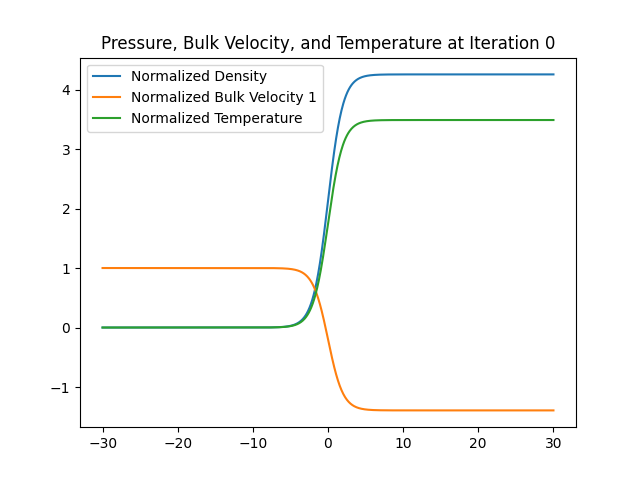
\includegraphics[width=\textwidth]{imgs/iter0.png}
        % \caption{Image 1}
        \label{fig:image1}
    \end{subfigure}
    \hfill
    \begin{subfigure}[b]{0.45\textwidth}
    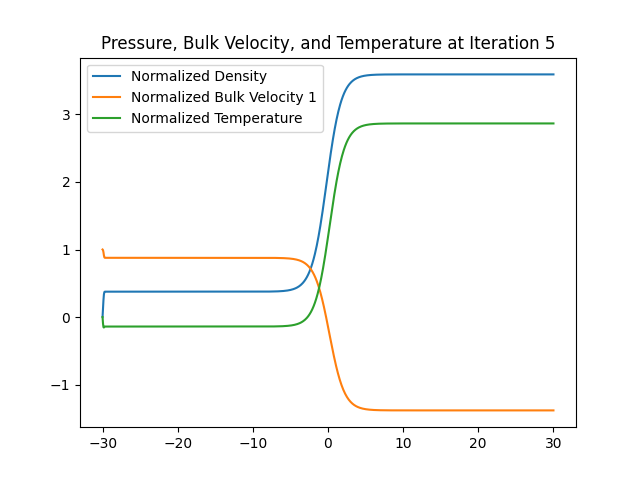
\includegraphics[width=\textwidth]{imgs/iter5.png}
        % \caption{Image 2}
        \label{fig:image2}
    \end{subfigure}
    
    \vspace{1em} % Add some vertical space between the rows
    
    \begin{subfigure}[b]{0.45\textwidth}
    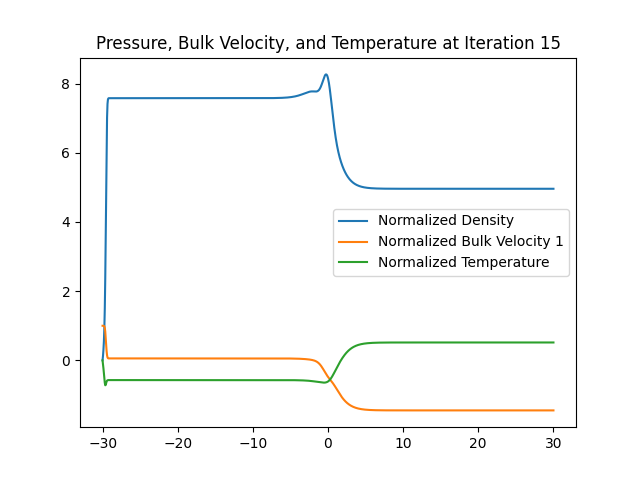
\includegraphics[width=\textwidth]{imgs/iter15.png}
        % \caption{Image 3}
        \label{fig:image3}
    \end{subfigure}
    \hfill
    \begin{subfigure}[b]{0.45\textwidth}
    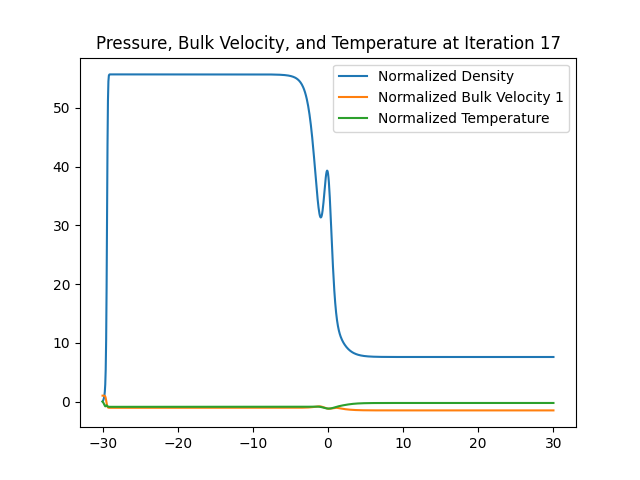
\includegraphics[width=\textwidth]{imgs/iter17.png}
        % \caption{Image 4}
        \label{fig:image4}
    \end{subfigure}
    
    \caption{These are the results from the time-stepping method. We see that the density function begins to grow without bound as time marches forward. This is similar to what occurs in the Lax-Friedrichs fast sweeping scheme that I implemented}
    \label{fig:four_images}
\end{figure}

I also had time to perform one sanity check this week. I removed the collision operator from the equation in order to see whether or not the solution simply advected to the right as it should. In other words, I modeled
\[
    \partial_t f + v \partial_x f = 0.
\]
I achieved exactly what I expected for this equation. The initial conditions simply moved to the left. This confirms what I had suspected: I am handling the collision operator incorrectly.
\section{To Do For Next Week}
It is clear that the collision operator is the source of my problems. I plan to revisit the implementation of the collision operator and determine why it misbehaving. I mentioned in the previous update that I altered Jingwei's code as seen below. 
\bigskip
\begin{lstlisting}
    def Qplus(f, N, R, L, Ntheta):
        """
        Carleman spectral method for the classical Boltzmann collision operator
        2D Maxwell molecule
        N # of Fourier modes: f(N,N), Q(N,N)
        theta: mid-point rule
        """
        temp = np.concatenate((np.arange(0,N//2),np.arange(-N//2,0,1)))
        l1 = np.array([[row]*N for row in temp])
        l2 = l1.T
        
        FTf = fft2(f)
    
        QG = np.zeros((N, N), dtype=np.complex_)
        bb = np.zeros((N, N), dtype=np.complex_)
    
        wtheta = np.pi / Ntheta
        theta = np.arange(wtheta / 2, np.pi, wtheta)
        sig1 = np.cos(theta)
        sig2 = np.sin(theta)
    
        for q in range(Ntheta):
            aa1 = alpha2(l1 * sig1[q] + l2 * sig2[q], R, L)
            aa2 = alpha2(np.sqrt(l1**2 + l2**2 - (l1 * sig1[q] + l2 * sig2[q])**2), R, L)
    
            QG += 2 * wtheta * ifft2(aa1 * FTf) * ifft2(aa2 * FTf)
            bb += 2 * wtheta * aa1 * aa2
    
        # Original code #################
        # QL = f * ifft2(bb * FTf)
        # Q = np.real(QG - QL)
        #################################
    
        # Adjusted code #################
        Q = np.real(QG)
        #################################
    
        return Q
    \end{lstlisting}
\bigskip
This is an inuitive way to change the method, but I have not actually done any analysis to ensure that this is correct thinng to do.
\end{document}
